\chapter{城市交通道路网络模拟}\label{ch:城市交通道路网络模拟}
在本案例学习过程中,对城市交通道路网络的构建采用开源平台Python + OpenStreetMap + Uber Movement。由于使用开源平台,因此对城市网络的构建是免费的,例如使用Google Maps API也可以构建道路网络,但是需要付费使用。此外Valhalla库也是开源的,可以作为备选项,但是Valhalla的学习曲线比较陡峭,需要花费大量时间和精力学习。基于上面的优缺点分析,选择使用Python中的Osmnx环境进行道路的构建模拟。


\section{Osmnx环境介绍与搭建}\label{sec:环境搭建}
OSMNX是一个Python软件包,可以从OpenStreetMap和模型,项目,可视化和分析现实世界中的街道网络以及任何其他地理空间几何形状下载地理空间数据。
可以使用Python代码下载并建模可步行,可驱动或骑自行车的城市网络,然后轻松分析和可视化它们。
也可以轻松地下载并使用其他基础设施类型,设施/兴趣点,建筑足迹,高程数据,街头轴承/方向以及速度/旅行时间。

由于Osmnx依赖于Anaconda,所以首先需要安装Anaconda环境,
然后使用conda config –prepend channel conda-forge和conda create -n ox –strict –channel-priority osmnx命令来创建osmnx环境。
安装完成后使用osmnx --version来检测osmnx环境是否安装成功,当在控制台出现osmnx的版本号时便表示环境搭建成功。

本文进行路网模拟测试实验所使用的环境为Python3.10 + Anaconda + OSMnx 1.1.2环境。


\section{数据准备}\label{sec:数据准备}
实验数据采用OpenStreetMap上获取的美国纽约市皇后区的街道道路信息和Uber Movement提供的相关的路段通行速度,部分数据信息见表\ref{tab:table}。
\begin{table}[H]
    \begin{center}
        \caption{纽约市皇后区城市道路信息(部分)}\label{tab:table}
        \begin{tabular}{llll}
            \hline
            id & osmWayId & hour & speed  \\
            \hline
            0  & 5029221  & 0    & 23.508 \\
            1  & 5029221  & 1    & 24.487 \\
            2  & 5029221  & 2    & 24.330 \\
            3  & 5029221  & 3    & 28.003 \\
            4  & 5029221  & 4    & 24.547 \\
            5  & 5029221  & 5    & 22.321 \\
            6  & 5029221  & 6    & 12.853 \\
            7  & 5029221  & 7    & 10.183 \\
            8  & 5029221  & 8    & 9.0898 \\
            9  & 5029221  & 9    & 11.414 \\
            10 & 5029221  & 10   & 12.677 \\
            11 & 5029221  & 11   & 12.395 \\
            12 & 5029221  & 12   & 13.598 \\
            13 & 5029221  & 13   & 13.382 \\
            14 & 5029221  & 14   & 13.656 \\
            15 & 5029221  & 15   & 11.505 \\
            \hline
        \end{tabular}
    \end{center}
\end{table}


\section{实验流程}\label{sec:实验流程}

\subsection{数据处理}\label{subsec:数据处理}
第一步需要根据街道道路信息创建道路网络,而OsMnx不仅可以对城市道路网络进行空间分析,同时也包含一系列用于创建道路网络和网络分析的函数。
其中包含由南加大规划系的Geoff Boeing教授编写的OpenStreetMap的python拓展增强包,
可以方便的进行城市道路网络的建模和对道路网络数据进行数据筛选,数据过滤,数据处理和数据分析。
借助这些工具包,配合OpenStreeMap可以很方便的构建出城市道路网络,并在其上进行城市道路网络状态的分析。

通过下面的代码首先可以创建出纽约市皇后区的城市道路网络,并对皇后区的城市道路网络数据
进行一个初步的过滤,程序中依据可达性分析的思想,避免边缘数据点对总体分布造成的极端影响,将连通节点数小于总节点数十分之一的部分节点看作为偏僻节点,其出行数据不作为最终结果的一部分。

\begin{lstlisting}[
    language=Python,
    morekeywords={as},
    label={lst:lstlisting5}
]
# 导入osmnx程序包
import osmnx as ox
# 构建纽约市皇后区城市道路网络图
G = ox.graph_from_place('Queens, New York, USA', network_type='drive')
# 准备一个列表, 用于存放待删除的边缘节点
remove_list = []
# 计算图中总的节点数量
num_nodes = len(G.nodes)
# 遍历图中的每一个节点, 计算其连通节点数量, 判断其是否为边缘节点
for node in G.nodes:
    # 计算当前节点的可达节点数
    reach = len(nx.descendants(G, node))
    # 判断可达节点数是否小于总节点数的1/10
    if reach < num_nodes / 10:
        # 如果是边缘节点, 则添加到列表中准备删除
        remove_list.append(node)
        # 删除所有的待删除节点
        for node in remove_list:
            G.remove_node(node)
            G = nx.convert_node_labels_to_integers(G, label_attribute='old_node_ID')
# 绘制出删除边缘节点后的城市道路网络图
ox.plot_graph(G)
\end{lstlisting}

\subsection{创建路网}\label{subsec:创建路网}
通过上面的数据处理,可以将获取到的每条街道的信息构建成一个交通网络,
其中包含表示每条街道交叉口的结点和表示每条街道各个方向的边。
同时由于该区域中网络结点数量多达19993个,街道数量更是达到542933条,
因此为了加快算法的收敛速度,选择将部分可达性较差的结点从网络中删除,
选择依据条件为:包含该结点的连通图中所含结点的数量小于总结点数量1/10的结点将会被从观察对象中剔除。
创建的纽约皇后区的路网对象如图\ref{fig:fig26}所示。

\begin{figure}[H] %H为当前位置,!htb为忽略美学标准,htbp为浮动图形
    \centering %图片居中
    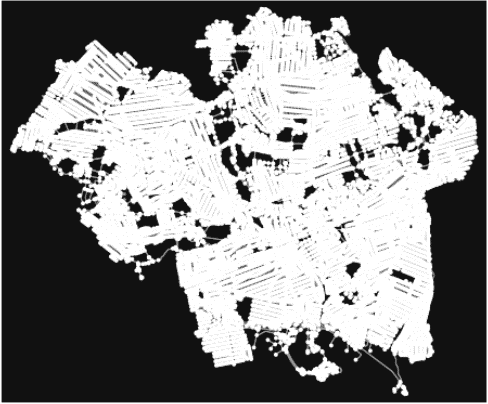
\includegraphics[width=0.7\textwidth]{png/图片26 纽约皇后区城市道路网} %插入图片,[]中设置图片大小,{}中是图片文件名
    \caption{纽约皇后区城市道路网} %最终文档中希望显示的图片标题
    \label{fig:fig26} %用于文内引用的标签
\end{figure}

\subsection{为路网附加时变行程时间}\label{subsec:为路网附加时变行程时间}
\begin{lstlisting}[
    language=Python,
    morekeywords={as},
    label={lst:lstlisting6}]
import osmnx as ox
import pandas as pd
# 为上面创建的纽约市皇后区的城市道路网络添加边属性
G = ox.add_edge_speeds(G)
# 为图中的边属性进行赋值, 保留小数点后一位
G = ox.speed.add_edge_travel_times(G, precision=1)
# 从OpenStreeMap下载的文件中读取道路网络中每一条边的最大行程速度
speed_df = pd.read_csv('nyc_avg_speeds_2019-06.csv')
# 根据距离和速度, 计算得到行程时间
speed_df = speed_df[['osm_way_id', 'hour', 'speed']]
speed_df.to_csv()
speed_dict = dict([((t.osm_way_id, t.hour), t.speed)
for t in speed_df.itertuples()])
speed_dict[(5029221, 12)]
\end{lstlisting}

为防止Uber提供的数据中没有直接给出路网的路段行程时间,
因此接下来通过已知的自由流的行程时间作为备用方案。
然后导入 Uber Movement 数据并转换为以 OSM Way ID 和一天中的小时为键的字典,
从而实现OpenStreetMap构建的路网的路段ID相匹配,并以一天为周期,
分别计算工作日内每个小时内的平均速度的平均值,得到路段通行速度,部分数据见表\ref{tab:table2},由于全部数据占用空间大,完整数据请通过附录\ref{ch:路网模拟实验代码}中代码生成。

\begin{table}[H]
    \caption{节点最短行程时间结果表(部分)}\label{tab:table2}
    \begin{tabular}{lllllllllllllllllllll}
        \hline
        & 0     & 1     & 2     & 3     & 4     & 5     & 6     & 7     & 8     & 9     \\
        \hline
        0  & 0.0   & 6.78  & 7.62  & 19.27 & 17.21 & 17.55 & 19.54 & 18.16 & 18.29 & 17.54 \\
        1  & 7.37  & 0.0   & 4.38  & 18.0  & 16.86 & 17.2  & 18.28 & 16.9  & 17.03 & 16.28 \\
        2  & 8.5   & 1.13  & 0.0   & 17.21 & 15.2  & 15.54 & 17.49 & 16.11 & 16.24 & 15.49 \\
        3  & 17.08 & 17.7  & 16.57 & 0.0   & 13.04 & 13.37 & 0.49  & 9.82  & 9.95  & 9.2   \\
        4  & 15.36 & 17.61 & 17.7  & 13.04 & 0.0   & 0.34  & 13.2  & 5.2   & 5.33  & 5.51  \\
        5  & 15.7  & 17.94 & 18.03 & 13.37 & 0.34  & 0.0   & 13.53 & 5.53  & 5.66  & 5.84  \\
        6  & 16.74 & 17.35 & 16.22 & 0.76  & 12.69 & 13.02 & 0.0   & 9.48  & 9.61  & 8.86  \\
        7  & 16.57 & 17.18 & 16.05 & 9.11  & 5.67  & 6.0   & 9.27  & 0.0   & 0.13  & 0.4   \\
        8  & 16.43 & 17.05 & 15.92 & 8.98  & 5.54  & 5.87  & 9.14  & 1.15  & 0.0   & 0.26  \\
        9  & 16.17 & 16.79 & 15.66 & 8.72  & 5.59  & 5.92  & 8.88  & 1.24  & 1.37  & 0.0   \\
        10 & 16.77 & 18.35 & 17.22 & 10.28 & 3.24  & 3.57  & 10.44 & 2.32  & 2.45  & 2.72  \\
        11 & 10.62 & 9.09  & 9.18  & 12.24 & 12.59 & 12.93 & 12.52 & 11.68 & 11.81 & 11.06 \\
        12 & 10.87 & 8.86  & 8.95  & 12.36 & 12.84 & 13.18 & 12.64 & 11.8  & 11.93 & 11.18 \\
        13 & 11.44 & 8.71  & 8.79  & 12.67 & 13.41 & 13.74 & 12.95 & 12.11 & 12.24 & 11.49 \\
        14 & 11.56 & 8.58  & 8.67  & 12.8  & 13.53 & 13.87 & 13.08 & 12.24 & 12.37 & 11.62 \\
        15 & 11.68 & 8.5   & 8.59  & 12.83 & 13.65 & 13.98 & 13.11 & 12.27 & 12.4  & 11.65 \\
        16 & 11.8  & 8.51  & 8.59  & 12.89 & 13.78 & 14.11 & 13.17 & 12.33 & 12.46 & 11.71 \\
        17 & 11.76 & 8.37  & 8.46  & 13.03 & 13.91 & 14.24 & 13.31 & 12.33 & 12.46 & 11.71 \\
        18 & 11.73 & 8.34  & 8.35  & 12.99 & 13.9  & 14.24 & 13.27 & 12.2  & 12.33 & 11.58 \\
        19 & 11.6  & 8.21  & 8.22  & 13.12 & 13.78 & 14.11 & 13.4  & 12.07 & 12.2  & 11.45 \\
        \hline
    \end{tabular}
\end{table}






